\begin{frame}
  \frametitle{MOOSE Framework}
  \begin{columns}
    \column[t]{6cm}
  \begin{figure}[t]
     \vspace{-0.25in}
       \hspace*{-0.25in}
       \includegraphics[height=0.65\textheight]{./images/moose.png}
            \caption{Multi-physics Object-Oriented Simulation Environment 
            (MOOSE) 
            \cite{gaston_physics-based_2015,permann2020moose,lindsay2021automatic}.}
  \end{figure}
        \column[t]{4cm}
          \begin{itemize}
                  \item Developed by Idaho National Laboratory 
                          \cite{gaston_physics-based_2015,permann2020moose,lindsay2021automatic}
                  \item Framework is truly open source (LGPL)
                  \item Accessible docs and tutorials at \url{https://mooseframework.inl.gov}
                  \item Source code at \url{https://github.com/idaholab/moose}
          \end{itemize}

  \end{columns}
\end{frame}



\begin{frame}
        \frametitle{MOOSE Apps \& Kernels}
  \begin{columns}
    \column[t]{6cm}
  \begin{figure}[t]
     \vspace{-0.25in}
       \hspace*{-0.25in}
       \includegraphics[height=0.65\textheight]{./images/moose.png}
            \caption{Multi-physics Object-Oriented Simulation Environment (MOOSE).}
  \end{figure}
        \column[t]{4cm}
          \textbf{Lots of Open Kernels}
           \footnotesize{\begin{itemize} 
                \item Chemical reactions
                \item Contact
                \item Fluid Properties
                \item Functional Expansion Tools
                \item Geochemistry
                \item Heat Conduction
                \item Level Set
                \item Navier-Stokes
                \item Peridynamics
                \item Phase Field
                \item Porous Flow
                \item Ray Tracing
                \item Reconstructed Discontinous Galerkin
                \item Tensor Mechanics
                \item \ldots
          \end{itemize}
          }
  \end{columns}
\end{frame}

\begin{frame}
        \frametitle{MOOSE Apps \& Kernels}
  \begin{columns}
    \column[t]{6cm}
  \begin{figure}[t]
     \vspace{-0.25in}
       \hspace*{-0.25in}
       \includegraphics[height=0.65\textheight]{./images/moose.png}
            \caption{Multi-physics Object-Oriented Simulation Environment (MOOSE).}
  \end{figure}
        \column[t]{4cm}
          \textbf{Lots of Open Apps}
           \begin{itemize} 
                   \item \href{https://github.com/arfc/moltres}{Moltres} (MSRs) \cite{lindsay_introduction_2019}
                   \item \href{https://github.com/arfc/squirrel}{Squirrel} (Utilities)
                   \item \href{https://github.com/idaholab/mastodon}{Mastodon} (structural dynamics, seismology)
                   \item \href{https://github.com/idaholab/pika}{pika} (microstructure)
                   \item \href{https://github.com/idaholab/falcon}{falcon}
                   \item \href{https://github.com/idaholab/blackbear}{blackbear}
                   \item \href{https://github.com/lcpp-org/crane}{crane} (plasma chemistry)
                   \item \href{https://github.com/casperversteeg/WhALE}{WhALE} (fluid-structure mechanics)
          \end{itemize}
  \end{columns}
\end{frame}

\begin{frame}
        \frametitle{MOOSE Apps \& Kernels}
  \begin{columns}
    \column[t]{6cm}
  \begin{figure}[t]
     \vspace{-0.25in}
       \hspace*{-0.25in}
       \includegraphics[height=0.65\textheight]{./images/moose.png}
            \caption{Multi-physics Object-Oriented Simulation Environment (MOOSE).}
  \end{figure}
        \column[t]{4cm}
          \textbf{Lots of Restricted Apps}\\
           \begin{itemize} 
                   \item BISON
                   \item Marmot
                   \item RattleSNake
                   \item Pronghorn
                   \item RELAP-7
                   \item \ldots 
          \end{itemize}
  \end{columns}
\end{frame}


\begin{frame}
        \frametitle{How Does it Work?}
  \begin{figure}
   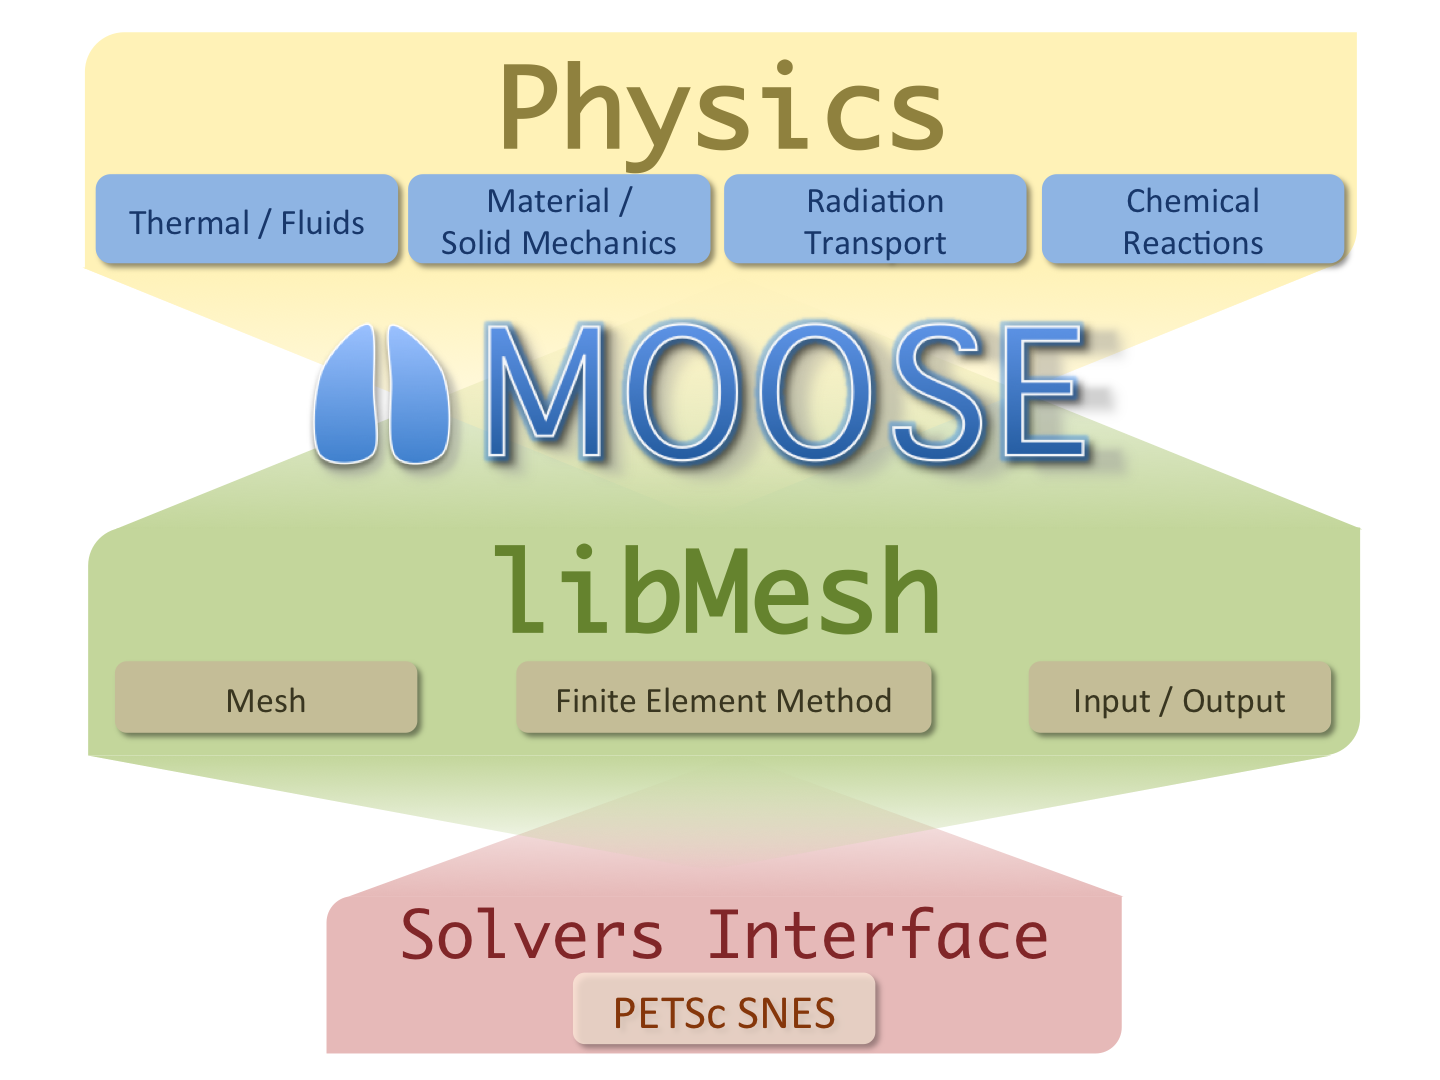
\includegraphics[height=0.8\textheight]{./images/moose_design.png}
          \caption{Shamelessly copied from the 
          \href{https://mooseframework.inl.gov/workshop/\#/2/4}{MOOSE Team Workshop slides}.}
    \end{figure}
\end{frame}


\begin{frame}
        \frametitle{How Does it Work?}
  \begin{figure}
   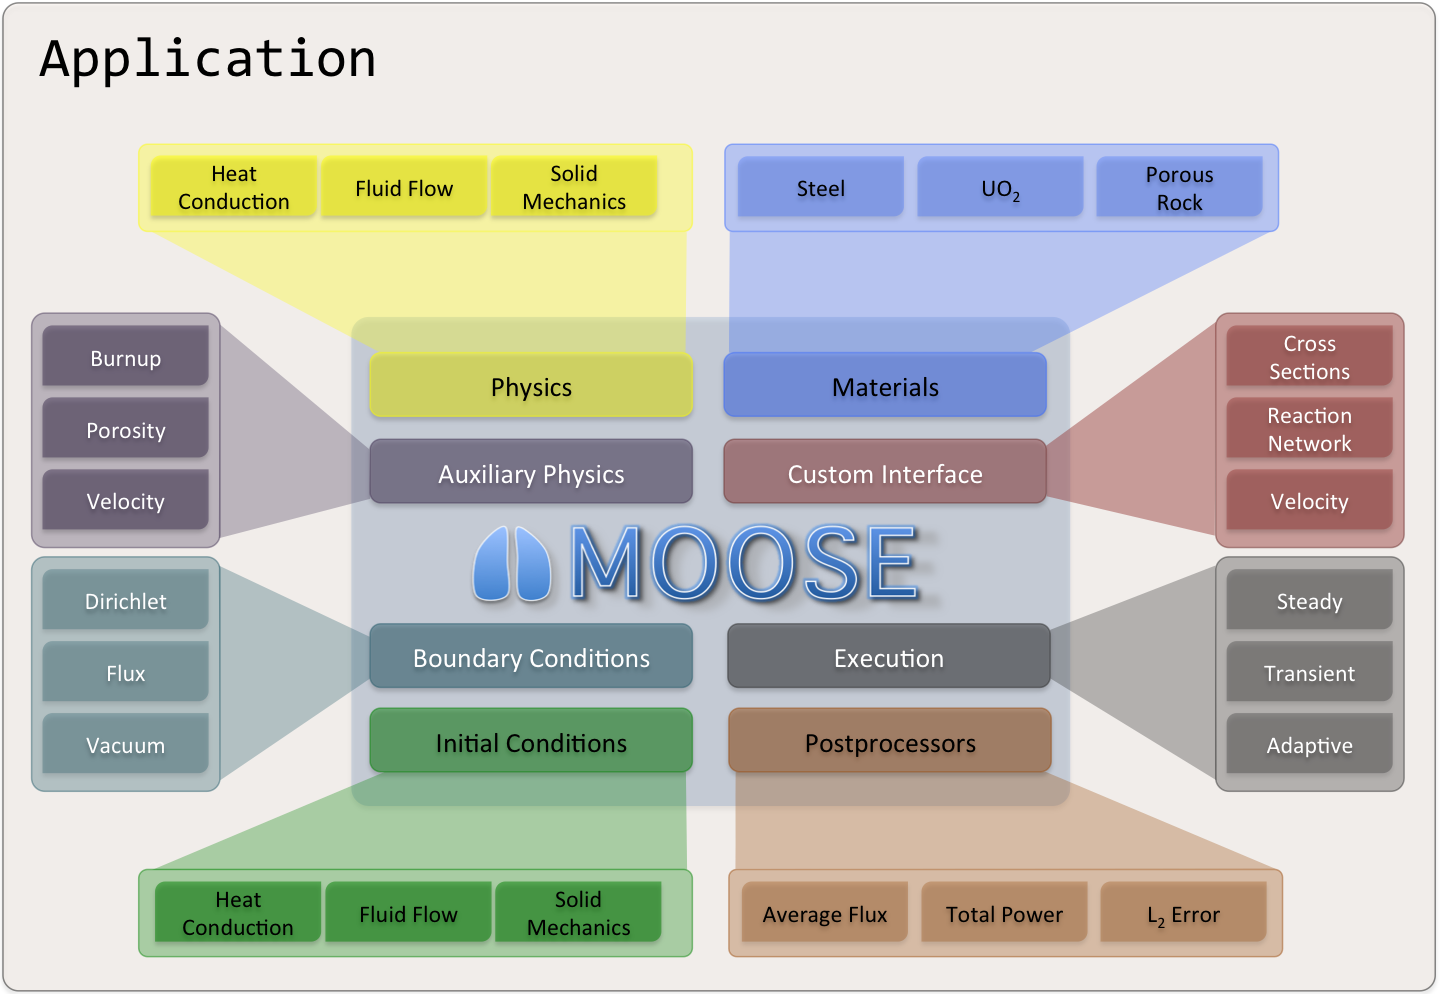
\includegraphics[width=0.9\textwidth]{./images/moose_systems.png}
          \caption{Shamelessly copied from the 
          \href{https://mooseframework.inl.gov/workshop/\#/2/6}{MOOSE Team Workshop slides}.}
    \end{figure}
\end{frame}

\begin{frame}
        \frametitle{How Does it Work?}
  \begin{figure}
   \vspace{-0.05in}
   \hspace*{-0.15in}
   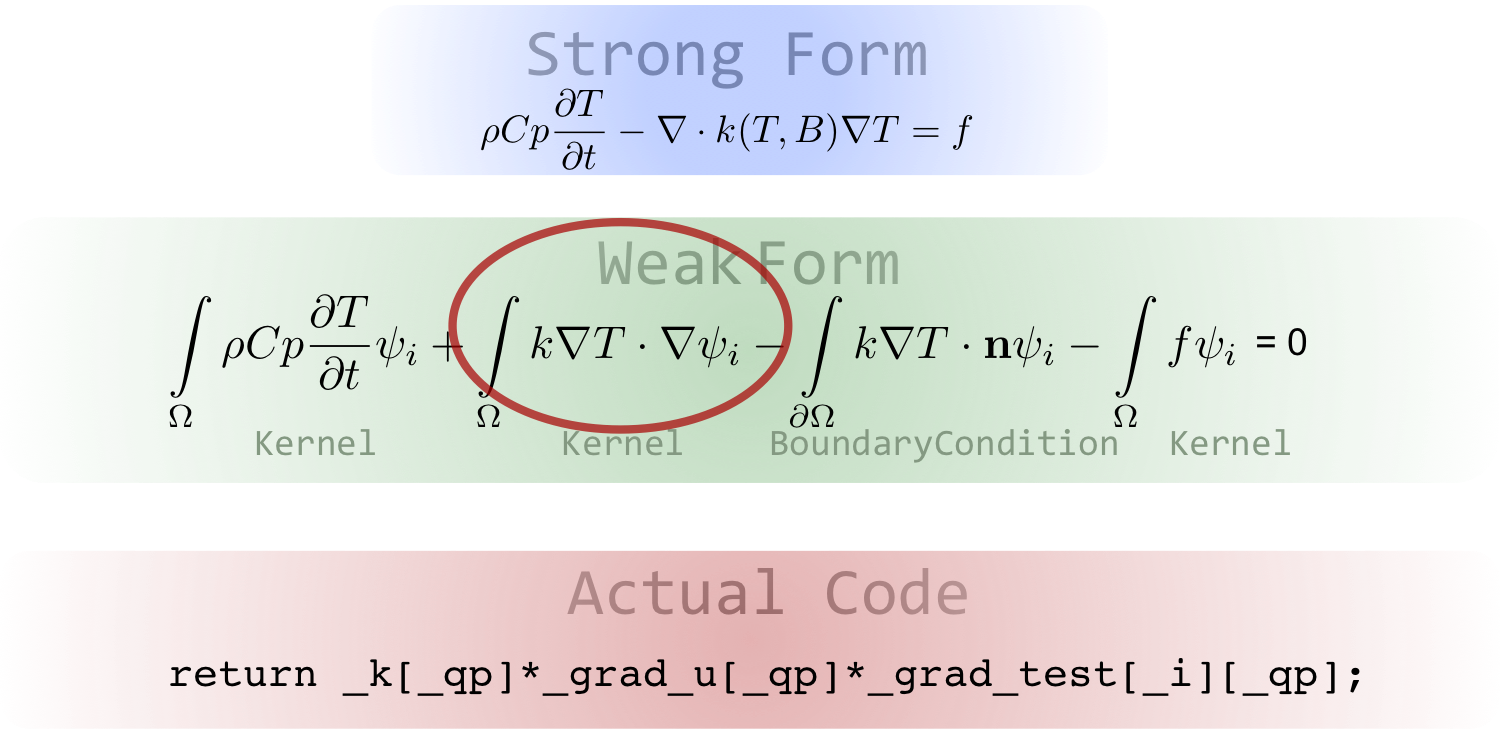
\includegraphics[width=\textwidth]{./images/moose_code.png}
          \caption{Shamelessly copied from the 
          \href{https://mooseframework.inl.gov/workshop/\#/2/7}{MOOSE Team Workshop slides}.}
    \end{figure}
\end{frame}

\begin{frame}
        \frametitle{MOOSE: Key Features}
        \begin{columns}
                \column[t]{5.5cm}
               \begin{itemize}
               \item MOOSE Framework is truly open source (LGPL)
               \item Developed initially for nuclear applications 
               \item Signficant long-term support from US DOE
               \item Continuous integration support (CIVET)
               \item Intuitive parallel multiscale solves
               \item Easy developer onboarding
               \end{itemize}
                \column[t]{5.5cm}
               \begin{itemize}
               \item Object Oriented, C++
               \item Interfaces with libMesh to discretize simulation volume into finite elements
               \item Residuals and Jacobians handed off to PetSc which handles solution of resulting non-linear system of algebraic equations
               \item Fully-coupled, fully-implicit multiphysics solver
               \item Automatically parallel (largest runs \textgreater 100,000 CPU cores!)
               \item Built-in adaptive meshing \& timestepping 
               \end{itemize}
        \end{columns}

\end{frame}

\begin{frame}
        \frametitle{Pros and Cons}
        \begin{columns}
                \column[t]{5.5cm}
                \textbf{Pros (+)}
               \begin{itemize}
               \item LGPL means the Framework is open, but apps can be restricted
               \item Vast array of available apps and kernels
               \item Many solver and preconditioning options
               \item Finite Element Modeling
               \item Full coupling is optional
               \item Generates gorgeous visualizations
               \end{itemize}
                \column[t]{5.5cm}
                \textbf{Cons (-)}
               \begin{itemize}
               \item LGPL means the Framework is open, but apps can be restricted
               \item Vast array of available apps and kernels
               \item Many solver and preconditioning options
               \item Finite Element Modeling
               \item Full coupling is optional
               \item Generates gorgeous visualizations
               \end{itemize}
        \end{columns}

\end{frame}

\section{Moltres (a MOOSE Application)}

\begin{frame}
        \frametitle{Moltres: Coupling in MOOSE}
  \begin{figure}
   \vspace{-0.05in}
   \hspace*{-0.15in}
   \includegraphics[width=1.1\textwidth]{./images/moltres-moose-diag.png}
    \end{figure}
\end{frame}


\begin{frame}
        \frametitle{Moltres: Basics}
        \begin{itemize}  
                \item Developed in ARFC group
                \item Fluid-fuelled, molten salt reactors
                \item Multi-group diffusion (arbitrary groups)
                \item Advective movement of delayed neutron precursors
                \item Navier-Stokes thermal hydraulics
                \item 3D unstructured
                \item 2D axisymmetric
                \item 3D structured 
                \item Initial developer: Alexander Lindsay \cite{lindsay_introduction_2018}
        \end{itemize}
\end{frame}

\begin{frame}
        \frametitle{Acquiring Moltres}
             \texttt{git clone https://github.com/arfc/moltres}\\
        \texttt{cd moltres}\\
        \texttt{git submodule init}\\
        \texttt{git submodule update}\\
\end{frame}

\begin{frame}
        \frametitle{Diffusion in Moltres}
        \footnotesize{
        \begin{align}
        \frac{1}{v_g}\frac{\partial \phi_g}{\partial t} &- \nabla \cdot D_g
        \nabla \phi_g + \Sigma_g^r \phi_g =\\
                &\sum_{g \ne g'}^G \Sigma_{g'\rightarrow g}^s \phi_{g'} + \chi_g^p \sum_{g' = 1}^G (1 -
        \beta) \nu \Sigma_{g'}^f \phi_{g'} + \chi_g^d \sum_i^I \lambda_i C_i
        \end{align}}
\begin{columns}
    \begin{column}{0.48\textwidth}
        \footnotesize{
        \begin{align*}
                v_g &= \mbox{speed of neutrons in group g} \\
                \phi_g &= \mbox{flux of neutrons in group g} \\
                t &= \mbox{time} \\
                D_g &= \mbox{Diffusion coefficient for neutrons in group g} \\
                \Sigma_g^r &= \mbox{macroscopic cross-section for}\\
                &\mbox{removal of neutrons from group g} \\
                \Sigma_{g'\rightarrow g}^s &= \mbox{macroscopic cross-section 
                of}\\
                &\mbox{  scattering from g' to g} \\
                \chi_g^p &= \mbox{prompt fission spectrum, neutrons in group g} \\
        \end{align*}}
    \end{column}
    \begin{column}{0.48\textwidth}
        %Content
        \footnotesize{
        \begin{align*}
                G &= \mbox{number of discrete groups, g} \\
                \nu &= \mbox{neutrons produced per fission} \\
                \Sigma_g^f &= \mbox{macroscopic fission cross section}\\
                &\mbox{ due to neutrons in group g} \\
                \chi_g^d &= \mbox{delayed neutrons in group g} \\
                I &= \mbox{ delayed neutron precursor groups} \\
                \beta &= \mbox{delayed neutron fraction}\\
                \lambda_i &= \mbox{average decay constant}\\
                &\mbox{of delayed neutron precursors in group i} \\
                C_i &= \mbox{concentration of delayed neutron}\\
                &\mbox{precursors in precursor group i}\\.
        \end{align*}}
    \end{column}
\end{columns}
\end{frame}

\begin{frame}
        \frametitle{Moltres Delayed Neutrons}
        \begin{align}
        \frac{\partial C_i}{\partial t} &= \sum_{g'= 1}^G \beta_i \nu
        \Sigma_{g'}^f \phi_{g'} - \lambda_i C_i - \frac{\partial}{\partial z} u
        C_i \label{eq:precursors}
\end{align}

        \begin{align*}
                G &= \mbox{number of discrete groups, g} \\
                I &= \mbox{ delayed neutron precursor groups} \\
                C_i &= \mbox{concentration of delayed neutron}\\
                &\mbox{precursors in precursor group i}\\.
                u &= \mbox{vertical fluid velocity}\\
                \lambda_i &= \mbox{average decay constant}\\
                &\mbox{of delayed neutron precursors in group i} \\
                \beta &= \mbox{fraction of delayed neutron}\\
                &\mbox{precursors in group i} \\
        \end{align*}
\end{frame}


\begin{frame}
        \frametitle{Moltres Fuel Temperature}
\begin{align}
        \rho_fc_{p,f}\frac{\partial T_f}{\partial t} &+ \nabla\cdot\left(\rho_f
        c_{p,f} \vec{u}\cdot T_f -k_f\nabla T_f\right) =  Q_f
\end{align}
\begin{align}
  \rho_f &= \mbox{density of fuel salt}\\
  c_{p,f} &= \mbox{specific heat capacity of fuel salt}\\
  T_f &= \mbox{temperature of fuel salt}\\
  \vec{u} &= \mbox{velocity of fuel salt}\\
  k_f &= \mbox{thermal conductivity of fuel salt}\\
  Q_f &= \mbox{source term} = \sum_{g=1}^G \epsilon_{f,g}\Sigma_{f,g}\phi_g
\end{align}
\end{frame}


\begin{frame}
        \frametitle{Moltres Moderator Temperature}
\begin{align}
        \rho_gc_{p,g}\frac{\partial T_g}{\partial t} &+
        \nabla\cdot\left(-k_g\nabla T_g\right) =  Q_g\\
\end{align}
\begin{align}
  \rho_g &= \mbox{density of graphite moderator}\\
  c_{p,g} &= \mbox{specific heat capacity of graphite moderator}\\
  T_g &= \mbox{temperature of graphite moderator}\\
  k_g &= \mbox{thermal conductivity of graphite moderator}\\
  Q_g &= \mbox{source term in graphite moderator}\\
\end{align}

\end{frame}


\begin{frame}
        \frametitle{Moltres MSRE Simulation}
  \begin{figure}
   \vspace{-0.05in}
   \includegraphics[height=0.85\textheight]{./images/msre.png}
    \end{figure}
\end{frame}


%\begin{frame}
%        \frametitle{Moltres MSRE Simulation}
%  \begin{figure}
%   \vspace{-0.05in}
%   \includegraphics[width=1.2\textwidth]{./images/moltres-input.png}
%          \caption{Data used in \cite{lindsay_introduction_2018}.}
%    \end{figure}
%\end{frame}

%\begin{frame}
%        \frametitle{Moltres MSRE Simulation}
%  \begin{figure}
%   \vspace{-0.05in}
%   \includegraphics[width=0.85\textwidth]{./images/moltres-composition.png}
%          \caption{Data used in \cite{lindsay_introduction_2018}.}
%    \end{figure}
%\end{frame}


\begin{frame}
        \frametitle{Mesh Generation for MOOSE Apps like Moltres}
  \begin{figure}
   \vspace{-0.05in}
   \includegraphics[height=0.85\textheight]{./images/lindsay_msre_moose.png}
    \end{figure}
\end{frame}



\begin{frame}
        \frametitle{Moltres Precursor Drift}
  \begin{figure}
   \vspace{-0.1in}
   \includegraphics[width=0.28\textwidth]{./images/auto_diff_rho_pre1.eps}
   \includegraphics[width=0.28\textwidth]{./images/auto_diff_rho_pre2.eps}
   \includegraphics[width=0.28\textwidth]{./images/auto_diff_rho_pre3.eps}
   \includegraphics[width=0.28\textwidth]{./images/auto_diff_rho_pre4.eps}
   \includegraphics[width=0.28\textwidth]{./images/auto_diff_rho_pre5.eps}
   \includegraphics[width=0.28\textwidth]{./images/auto_diff_rho_pre6.eps}
    \end{figure}
\end{frame}




\begin{frame}
        \frametitle{Moltres: More Complex Mesh}
  \begin{figure}[t]
   \vspace{-0.1in}
   \hspace*{-0.45in}
   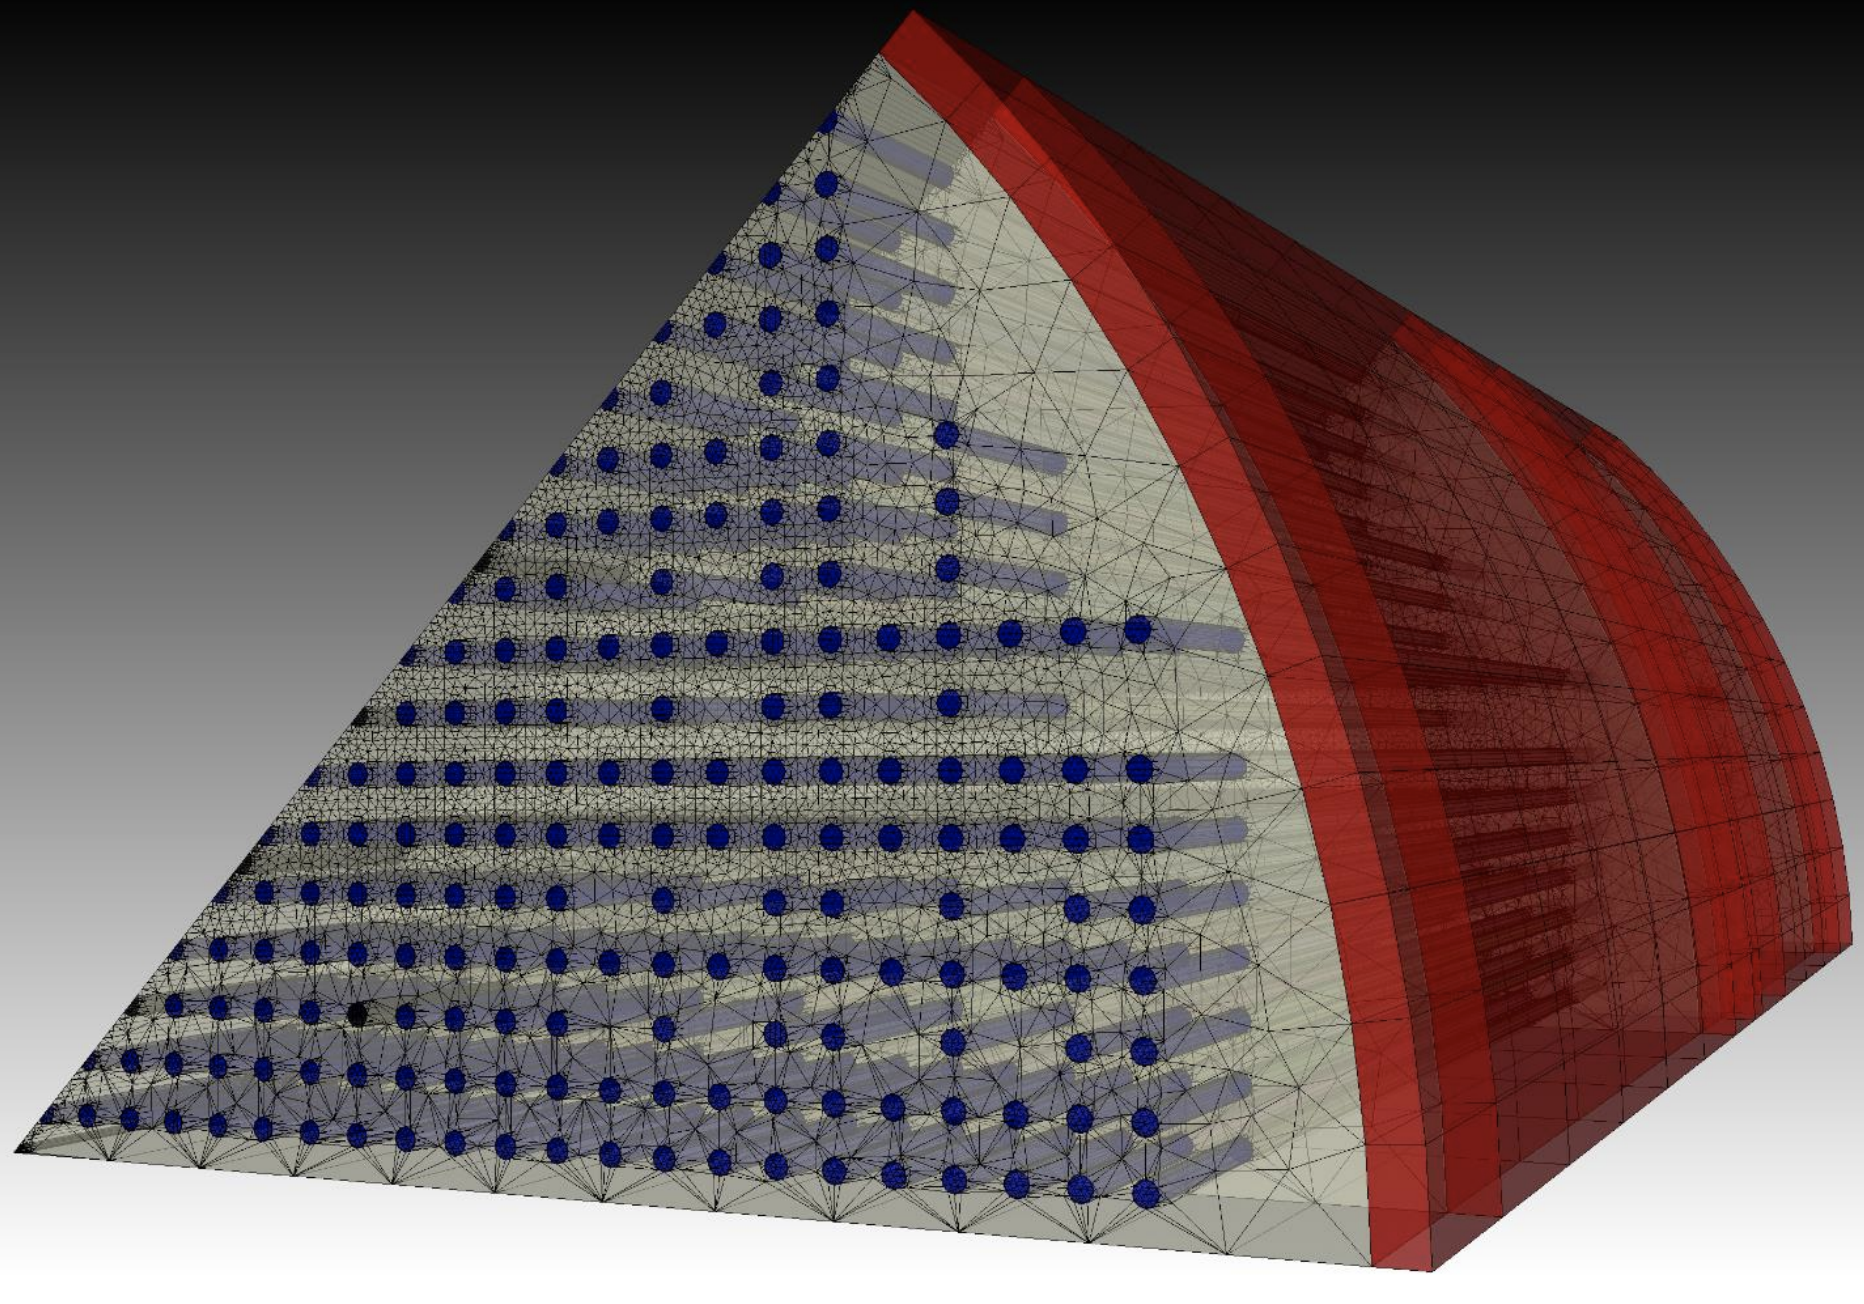
\includegraphics[height=0.75\textheight]{./images/lee-tap-mesh.png}
          \caption{TAP Mesh generated by Alvin Lee \cite{lee_neutronics_2020}. Red = Reactor Vessel Wall, Light Yellow =
Fuel Salt, Dark Gray = Control Rods, Blue = Fuel Salt radially co-located with 
          the Moderator Rods.}
    \end{figure}

\end{frame}

\begin{frame}
  \frametitle{Moltres: Multiphysics simulation (3D)}
  \begin{figure}[t]
   \vspace{-0.1in}
   \hspace*{-0.45in}
   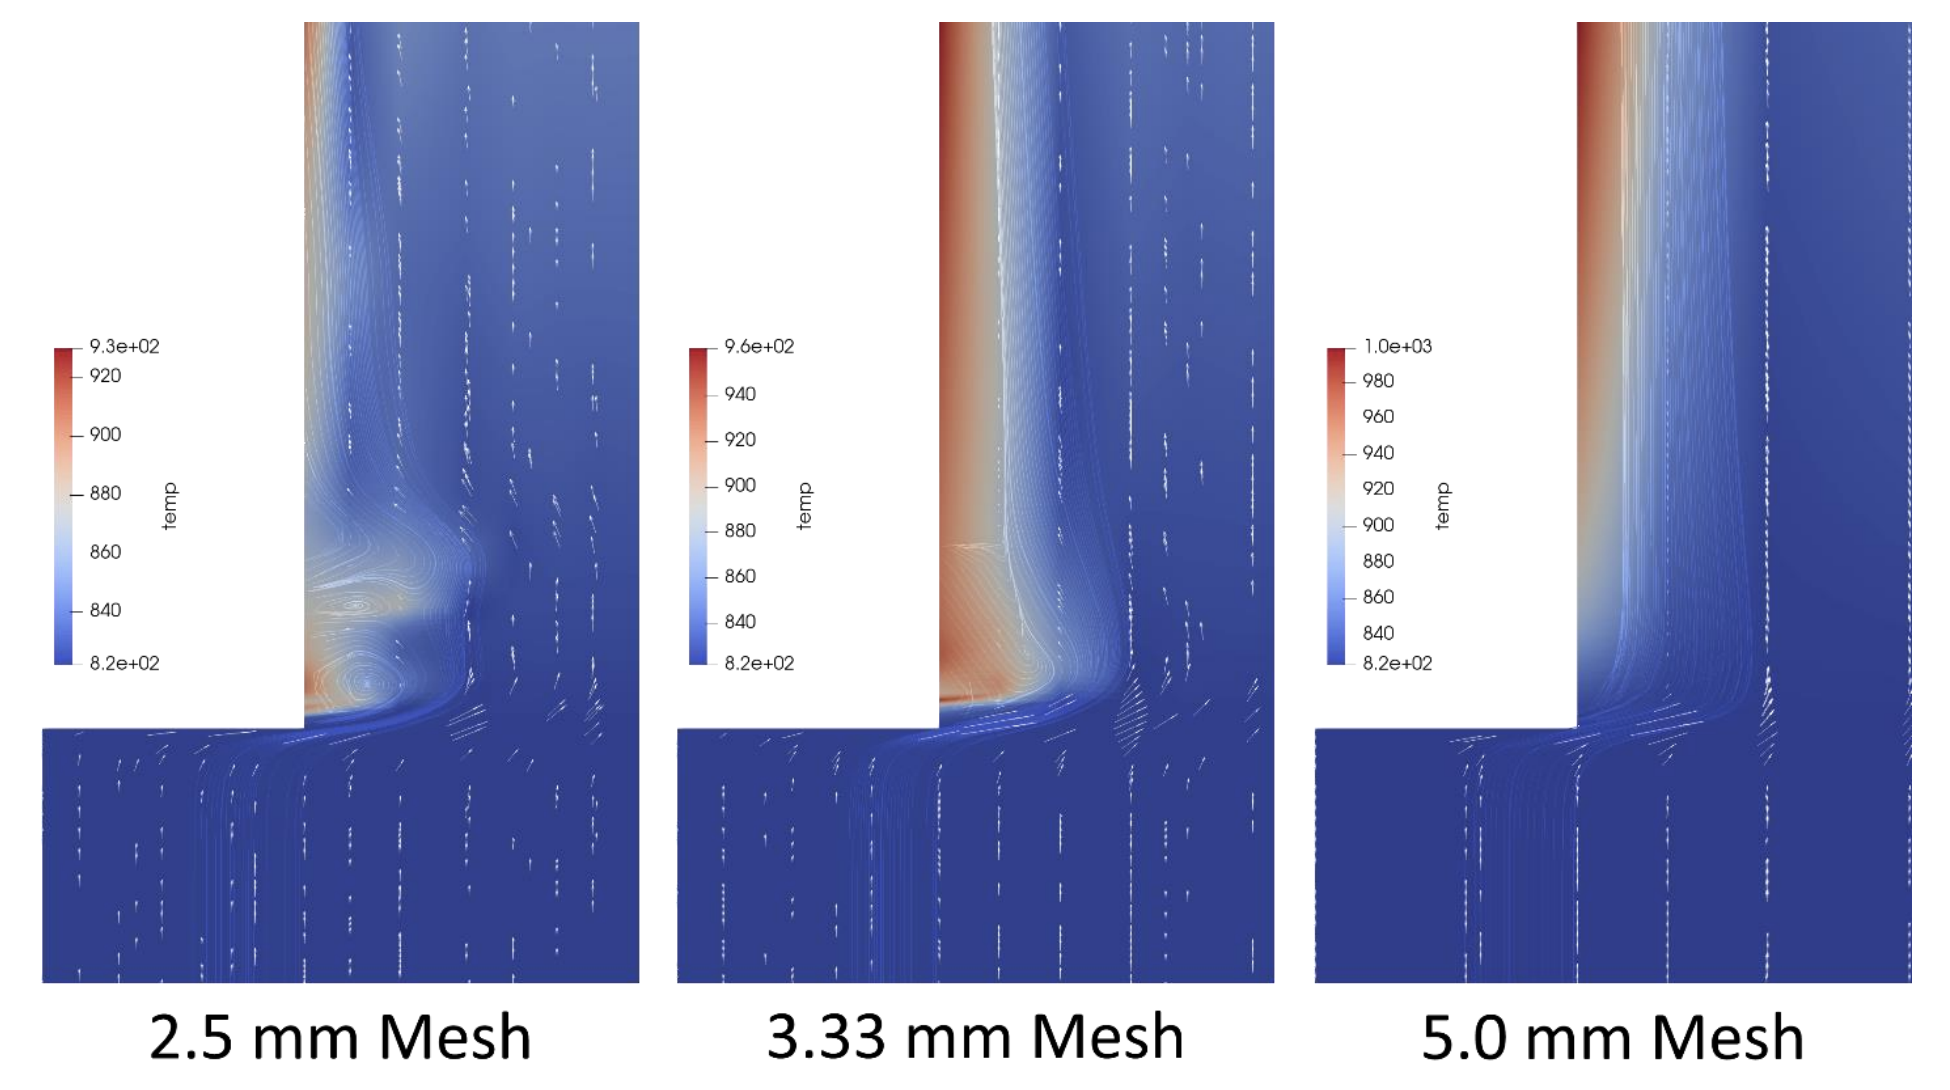
\includegraphics[height=0.75\textheight]{./images/lee-instability-resolution.png}
          \caption{Meshing study by Alvin Lee \cite{lee_neutronics_2020} 
          regarding KH instabilities and resolution of MSR fuel salt vortices.}
    \end{figure}

\end{frame}

\begin{frame}
        \frametitle{What now?}
        \textbf{Get Started}\\
        \href{https://mooseframework.inl.gov/}{https://mooseframework.inl.gov/}
        \href{https://github.com/idaholab/moose}{https://github.com/idaholab/moose}\\
        \href{https://github.com/arfc/moltres}{https://github.com/arfc/moltres}\\
        \textbf{Other Tools}\\
        \href{https://gmsh.info/}{https://gmsh.info}\\
        \href{https://github.com/pyne/pyne}{https://github.com/pyne/pyne}\\
        \href{https://github.com/openmc-dev/openmc}{https://github.com/openmc-dev/openmc}\\
        \href{https://www.paraview.org}{https://www.paraview.org}

\end{frame}
